\subthesischapter{Definición de los casos de uso}
\subsubthesischapter{Identificación de los actores}
Los actores no son parte del sistema, pero sí pueden intercambiar información con él, ellos representan un rol que juegan una o varias personas, un equipo o un sistema automatizado. En la aplicación de juego serio se identificaron los siguientes actores:

\begin{table}[ht]
    \centering
    \begin{tabularx}{\textwidth}{|l|X|}
        \hline
        \textbf{Actores} & \textbf{Descripción} \\\hline
        Usuario & Individuo que interactúa con el sistema para hacer uso de una rutina de entrenamiento
        como medio de rehabilitación, diversión o entrenamiento físico \\\hline
        Sistema & Es la misma aplicación que en determinadas ocasiones ejecuta funcionalidades automáticamente producto de la interacción con el pedal motorizado. \\\hline
    \end{tabularx}
    \label{tab: actores}
    \caption{Descripción de actores}
\end{table}

\subsubthesischapter{Identificación de los casos de usos}    
Cada forma en que los actores usan el sistema se representa con un caso de uso, como fragmentos de funcionalidad que el sistema ofrece para aportar solución a la necesidad de esta aplicación. Los casos de uso que se definen para el sistema propuesto están reflejados en la tabla \ref{tab: rf} con su respectivo diagrama en las figura \ref{fig: use-cases-user} y \ref{fig: use-cases-system}.
\begin{table}[ht]
    \centering
    \begin{tabularx}{\textwidth}{|c|X|c|}
        \hline
        \textbf{Casos de uso} & \textbf{Descripción} & \textbf{Requisitos}\\\hline
        Iniciar sesión & Permite al usuario acceder al sistema & RF1\\\hline
        Registrar usuario & Permite guardar los datos de un usuario en la Base de Datos & RF2\\\hline
        Eliminar usuario & Permite eliminar la cuenta de un usuario en la Base de Datos & RF3\\\hline
        Editar datos del usuario & Permite actualizar los datos personales del usuario en la Base de Datos & RF4\\\hline
        Cerrar sesión & Permite al usuario cerrar sesión en el sistema & RF5\\\hline
        Enviar datos al pedal & Permite a la aplicación enviar datos al pedal & RF6 \\\hline
        Recibir datos del pedal & Permite a la aplicación recibir los datos provenientes del pedal & RF7\\\hline
        Establecer comunicación & Permite establecer comunicación entre el dispositivo Android y el Pedal Motorizado & RF8\\\hline
        Finalizar Comunicación & Permite finalizar comunicación entre el dispositivo Android y el Pedal Motorizado & RF9\\\hline
        Iniciar rutina & Permite dar inicio a la rutina de entrenamiento & RF10\\\hline
        Pausar/Reanudar rutina & Permite pausar la etapa actual de la rutina & RF11\\\hline
        Finalizar rutina & Permite dar fin a la rutina de entrenamiento & RF12\\\hline
        Mostrar estadística & Permite mostrar estadísticas de las rutinas de entrenamiento  al usuario& RF13\\\hline
        Configurar rutina & Permite elegir la modalidad e insertar los parámetros de la rutina  & RF14\\\hline
        Iniciar calibración & Permite iniciar la calibración para la modalidad clínica  & RF15\\\hline
        Guardar logs & Permite almacenar los hechos ocurridos en el sistema en ficheros de logs & RF16\\\hline
        %Iniciar juego rutina libre & Permite dar inicio a la rutina de entrenamiento libre \\\hline
        %Iniciar juego rutina resistido & Permite dar inicio a la rutina de entrenamiento resistido \\\hline
    \end{tabularx}
    \caption{Casos de uso del sistema}
    \label{tab: rf}
\end{table}
    
\vspace*{50pt}
\begin{figure}[h]
    \centering
    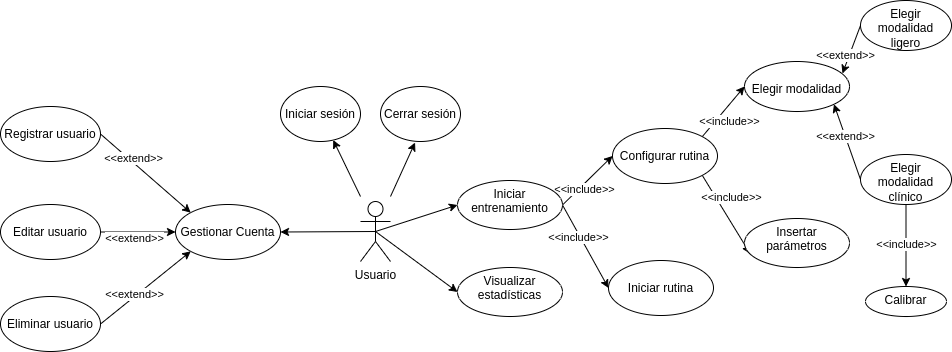
\includegraphics[scale=0.44]{images/diagram-usecase-user.png}
    \caption{Diagrama de casos de uso, actor usuario}
    \label{fig: use-cases-user}
\end{figure}

\vspace*{50pt}
\begin{figure}[h]
    \centering
    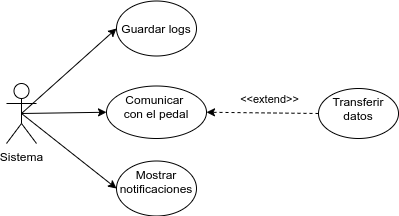
\includegraphics[scale=0.44]{images/diagram-usecase-system.png}
    \caption{Diagrama de casos de uso, actor sistema}
    \label{fig: use-cases-system}
\end{figure}